\documentclass[amsmath,amssymb,twocolumn,superscriptaddress]{revtex4-1}

\usepackage{graphicx}% Include figure files
\usepackage{dcolumn}% Align table columns on decimal point
\usepackage{bm}% bold math
\usepackage[detect-all]{siunitx}
\usepackage{hyperref}% add hypertext capabilities
\usepackage{xr}
\usepackage{mhchem}
\graphicspath{{./figures/}}


\begin{document}                  % DO NOT DELETE THIS LINE

\title{Applying molecular simulation to the analysis of lipid monolayer reflectometry}

\author{A.~R. McCluskey}
\email{a.r.mccluskey@bath.ac.uk}
\affiliation{Department of Chemistry, University of Bath, Claverton Down,
Bath, BA2 7AY, UK}
\affiliation{Diamond Light Source, Harwell Campus, Didcot, OX11 0DE, UK}

\author{J. Grant}
\affiliation{Computing Services, University of Bath, Claverton Down, Bath, BA2 7AY, UK}

\author{A. J. Smith}
\affiliation{Diamond Light Source, Harwell Campus, Didcot, OX11 0DE, UK}

\author{J. L. Rawle}
\affiliation{Diamond Light Source, Harwell Campus, Didcot, OX11 0DE, UK}

\author{D. J. Barlow}
\affiliation{Institute of Pharmaceutical Science, King's College London, London, SE1 9NH, UK}

\author{M. J. Lawrence}
\affiliation{Division of Pharmacy and Optometry, University of Manchester, Manchester, M13 9PT, UK}

\author{S.~C. Parker}
\affiliation{Department of Chemistry, University of Bath, Claverton Down,
Bath, BA2 7AY, UK}

\author{K.~J. Edler}
\email{k.edler@bath.ac.uk}
\affiliation{Department of Chemistry, University of Bath, Claverton Down,
Bath, BA2 7AY, UK}

\date{\today}

\begin{abstract}
Using molecular simulation to aid in the analysis of neutron reflectometry measurements is commonplace.
However, reflectometry is a tool to probe large-scale structures, and therefore the use of all-atom simulation may be unjustified.
This work presents the first direct comparision between the reflectometry profiles obtained from different all-atom and coarse-grained molecular dynamics simulations.
These are compared with a traditional layer model analysis method to determine the minimum simulation resolution required to accurately reproduce experimental data.
We find that systematic problems limit the efficacy of the MARTINI potential model, while the Berger united-atom and Slipids all-atom potential models agree similarly well with the experimental data.
The traditional layer model gives the best agreement, however the higher resolution simulation-dependent methods produce agreement that is only slightly worse.
\end{abstract}

\maketitle                        % DO NOT DELETE THIS LINE

\section{Introduction}

Neutron and X-ray reflectometry techniques are popular in the study of nanolayered structures, such as polyelectrolyte-surfactant mixtures \cite{Llamas2018}, lipid bilayer systems \cite{Waldie2018}, electrodeposited films \cite{Beebee2019}, and dye-sensitised solar cell materials \cite{McCreeGrey2015}.
Unlike other surface-sensitive techniques, such as atomic force microscopy (AFM) or scanning electron microscopy (SEM), reflectometry methods can investigate buried interfaces in addition to the material surface.
This is due to the ability of neutrons and X-rays to probe more deeply into a material than an AFM tip or the electron.
Additionally, reflectometry techniques can more easily provide information about the average structure of a material over large regions of space, resulting in significantly improved sampling, compared with microscopy techniques \cite{Renaud2009}.

The growth in popularity of reflectometry techniques can be attributed to the significant development of reflectometry instrumentation, such as FIGARO, the horizontal neutron reflectometer at the ILL \cite{Campbell2011}, and the beam deflection system at the I07 beamline of the Diamond Light Source \cite{Arnold2012}.
These have enabled the study of more complex systems including biomimetic bacterial membrane \cite{Barker2016}, and polymeric energy materials \cite{Khodakarimi2016}.
However, the ability to study complex systems poses an important data analysis challenge, where a typical layer model approach may not be sufficient.

The Abel\`{e}s matrix formalism for stratified media \cite{Abeles1950}, is the most commonly applied method to analyse reflectometry data from a surfactant monolayer.
This model-dependent approach involves the construction of a layer model to describe the system under study.
The reflectometry profile is then calculated from the model, and the model refined to improve agreement between the calculated reflectometry profile and that measured experimentally.
Such an approach is discussed in detail in the work of Campbell \emph{et al.} \cite{Campbell2018}, where they investigate the different approaches to the analysis of surfactant monolayers.

The Abel\`{e}s matrix formalism is often described as the dynamical approach to reflectometry analysis, in contrast to the Fourier transform-based kinematic approach \cite{Crowley1991,Lu1996}.
The dynamical approach considers the reflection and refraction of the probing radiation at a series of interfaces, where the refractive index is a function of the scattering length densities (SLDs) for each layer.
By considering Figure \ref{fig:dyn} it is clear how the reflected radiation could interact coherently and incoherently by analogy with Bragg's law.
%
\begin{figure}[h]
\centering
  \includegraphics[width=0.48\textwidth]{reflrefr}
  \caption{A schematic of a reflectometry experiment, where $i$ is the incident radiation, $r$ is the reflected radiation, $t$ is the transmitted radiation, and $d$ is the layer thickness, for each layer $n$, and the angles of incidence, reflection, and transmittence all depend on Snell's law.}
  \label{fig:dyn}
\end{figure}
%

A commonly suggested method for the multi-modal analysis of reflectometry measurements is the use of molecular dynamics (MD) simulations.
MD-driven multi-modal analysis has been applied previously, either by the calculation of the SLD profile from the simulation or the full determination of the reflectometry profile.
In the former case, the calculated SLD profile may be compared with the SLD profile determined from the use of a traditional analysis method.
Bobone \emph{et al.} used such a method to study the antimicrobial peptide trichogin GA-IV within a supported lipid bilayer \cite{Bobone2013}.
A four layer model consisting of the hydrated \ce{SiO2} layer, an inner lipid head-region, a lipid tail-region, and an outer lipid head region was used in the Abel\`{e}s matrix formalism.
The SLD profile from the MD simulations agreed well with that fitted to the reflectometry data from the layer model.

The reflectometry profile was calculated explicitly from classical simulation in the works of Miller \emph{et al.} and Anderson and Wilson \cite{Miller2003,Anderson2004}.
In these, an amphiphilic polymer at the oil-water interface was simulated by Monte Carlo and MD respectively, and the neutron reflectometry profile for found by splitting the simulation cell into a series of small layers and applying the Abel\`{e}s matrix formalism.
There was good agreement between the experimental and calculated reflectometry, for low interface coverages of the polymer.
Another work that has made direct comparison between the atomistic simulation-derived reflectometry and those measured experimentally includes that of Darr\'{e} \emph{et al.} \cite{Darre2015}.
In this work, NeutronRefTools was developed to produce the neutron reflectometry profile from a given MD simulation.
The particular system studied was a supported 1,2-dimyristoyl-\emph{sn}-glycero-3-phosphocholine (DMPC) lipid bilayer, with good agreement found between the simulation-derived profile and the experimental measurement.
However, the nature of the support required a correction for the head-group hydration to be imposed to achieve this agreement.

Koutsioubas used the MARTINI coarse-grained representation of a 1,2-dipalmitoyl-\emph{sn}-glycero-3-phosphocholine (DPPC) lipid bilayer to compare with experimental reflectometry \cite{Koutsioubas2016}.
This work shows that the parameterisation of the MARTINI water bead was extremely important in the reproduction of the reflectometry data, as the non-polarisable water bead would freeze into crystalline sheets resulting in artefacts in the reflectometry profiles calculated.
The work of Hughes \emph{et al.} studied again a DPPC lipid bilayer system \cite{Hughes2016}, albeit an all-atom representation, that was compared with a supported DPPC lipid bilayer system measured with polarised neutron reflectometry.
The SLD profile found from MD was varied to better fit the experimental measurement, resulting in good agreement.
Additionally, the variation of the SLD profile was used to remove artefacts that arose from poor splicing between the MD simulations that the layer model used in regions such as the gold and magnetic permalloy layers not present in the simulation.

In all of the examples discussed so far there is no direct comparison between the reflectometry profile determined from simulation and that from the application of a traditional analysis method.
Indeed, the only example, to the authors' knowledge where direct comparison was drawn is the work of Dabkowska \emph{et al.} \cite{Dabkowska2014}.
This work compares the reflectometry profile from a DPPC monolayer at the air-water interface containing dimethyl sulfoxide molecules with a similar molecular dynamics simulation parameterised with the CHARMM potential model.
The use of multimodal analysis allowed the determination of the position of a concentration of DMSO molecules at a particle region within a monolayer and the orientation of such molecules.

Herein, we present the comparison of three MD simulations of different potential models, with different particle grain-sizes; namely the Slipid all-atom \cite{Jambeck2012}, Berger united-atom \cite{Berger1997}, and MARTINI coarse-grained potential models \cite{Marrink2007}.
We believe that this work offers a fundemental insight into the simulation resolution that is required to reproduce experimental neutron reflectometry measurements.
Furthermore, we suggest some adjustments that may be made to the more traditional, layer models that are commonly used to analyse such measurements.

\section{Methodology}

\subsection{Neutron reflectometry measurements}
The neutron reflectometry measurements analysed in this work have been previously published by Hollinshead \emph{et al.} \cite{Hollinshead2009}, and full details of the methods used can be found in the previous publication.
These measurements involved studying seven contrasts of 1,2-distearoyl-\emph{sn}-phosphatidylcholine (DSPC) at the air-water interface (Table \ref{tbl:nom}), at four different surface pressures; \SIrange{20}{50}{\milli\newton\per\meter}.
%
\begin{table}[h]
\small
  \caption{\ The different contrasts of lipid and water investigated in this work. ACMW is air-contrast matched water, where \ce{D2O} and \ce{H2O} are mixed so as to given a water with a SLD of zero.}
  \label{tbl:nom}
  \begin{tabular*}{0.48\textwidth}{@{\extracolsep{\fill}}lll}
    \hline
    Shorthand & Lipid contrast & Water contrast \\
    \hline
    h-\ce{D2O} & h-DSPC & \ce{D2O} \\
    \ce{d_{13}}-ACMW & \ce{d_{13}}-DSPC & ACMW \\
    \ce{d_{13}}-\ce{D2O} & \ce{d_{13}}-DSPC & \ce{D2O} \\
    \ce{d_{70}}-ACMW & \ce{d_{70}}-DSPC & ACMW \\
    \ce{d_{70}}-\ce{D2O} & \ce{d_{70}}-DSPC & \ce{D2O} \\
    \ce{d_{83}}-ACMW & \ce{d_{83}}-DSPC & ACMW \\
    \ce{d_{83}}-\ce{D2O} & \ce{d_{83}}-DSPC & \ce{D2O} \\
    \hline
  \end{tabular*}
\end{table}
%

\subsection{Molecular dynamics simulations}
The DSPC monolayer simulations were made up of lipid molecules modelled with three potential models, each of a different particle grain-size.
The Slipids potential model is an all-atom representation of the lipid molecules \cite{Jambeck2012}, which was used alongside the single point charge (SPC) water model \cite{Berendsen1987}, with a timestep of \SI{0.5}{\femto\second}.
The Berger potential model is obtained by the integration of the hydrogen atoms to produce a united atom potential model \cite{Berger1997}; again the SPC water molecules were used.
The removal of the high frequency \ce{C-H} bonds allows for the timestep to be increased to \SI{1}{\femto\second}.
Finally, the lowest resolution potential model used was the MARTINI \cite{Marrink2007} alongside the polarisable MARTINI water model \cite{Yesylevskyy2010}, to avoid the freezing issues observed previously \cite{Koutsioubas2016}.
The MARTINI 4-to-1 heavy atom beading allows for the use of a \SI{20}{\femto\second} timestep.
All simulations were conducted with temperature coupling to a heat bath at \SI{300}{\kelvin} and a leap-frog integrator, and run using GROMACS 5.0.5 \cite{Berendsen1995,Lindahl2001,vanderSpoel2005,Hess2008} on 32 cores of the STFC Scientific Computing resource SCARF.
The simulation was of a monolayer, therefore the Ewald 3DC correction was applied to allow for the use of \emph{x}/\emph{y}-only periodic boundary conditions \cite{InChul1999}.
A close-packed ``wall'' of non-interacting dummy atoms was placed at each side of the simulation cell in the \emph{z}-direction to ensure that the atoms could not leave the simulation cell.

The starting simulation structure was generated using the molecular packing software Packmol \cite{Martinez2009}.
This was used to produce a monolayer of 100 DSPC molecules, with the head group oriented to the bottom of the simulation cell.
A \SI{6}{\angstrom} layer of water was then added such that the head groups were overlapping, this was achieved using the \texttt{solvate} functionality in GROMACS 5.0.5.
Examples of the dry and wet monolayer can be seen in Figure \ref{fig:drywet} for the Berger potential model system.
A general protocol was then used to relax the system at the desired surface coverage, reproducing the effects of a Langmuir trough \emph{in silico}.
This involved subjecting the system to a semi-isotropic barostats, with a compressibility of \SI{4.5E-5}{\per\bar} of the Slipids and Berger simulations and \SI{3.0E-4}{\per\bar} for the MARTINI simulations.
The pressure in the \emph{z}-dimension was kept constant at \SI{1}{\bar}, while it was increased in the \emph{x}- and \emph{y}-dimensions isotropically.
When the \emph{xy}-surface area is reached that is associated with the area per molecule (APM) for each surface pressure, described by the experimental surface pressure-isotherm (Figure \ref{fig:iso}), given in Table \ref{tbl:apm}, the coordinates were saved and used as the starting structure for the equilibration simulation.
This involved continuing the use of the semi-isotropic barostat, with the \emph{xy}-area of the box fixed, allowing the system to relax at a pressure of \SI{1}{\bar} in the \emph{z}-dimension.
The equilibration period was \SI{1}{\nano\second}, following which the \SI{50}{\nano\second} NVT ensemble production simulations were run, on which all analyses were conducted.
%
\begin{figure}[h]
\centering
  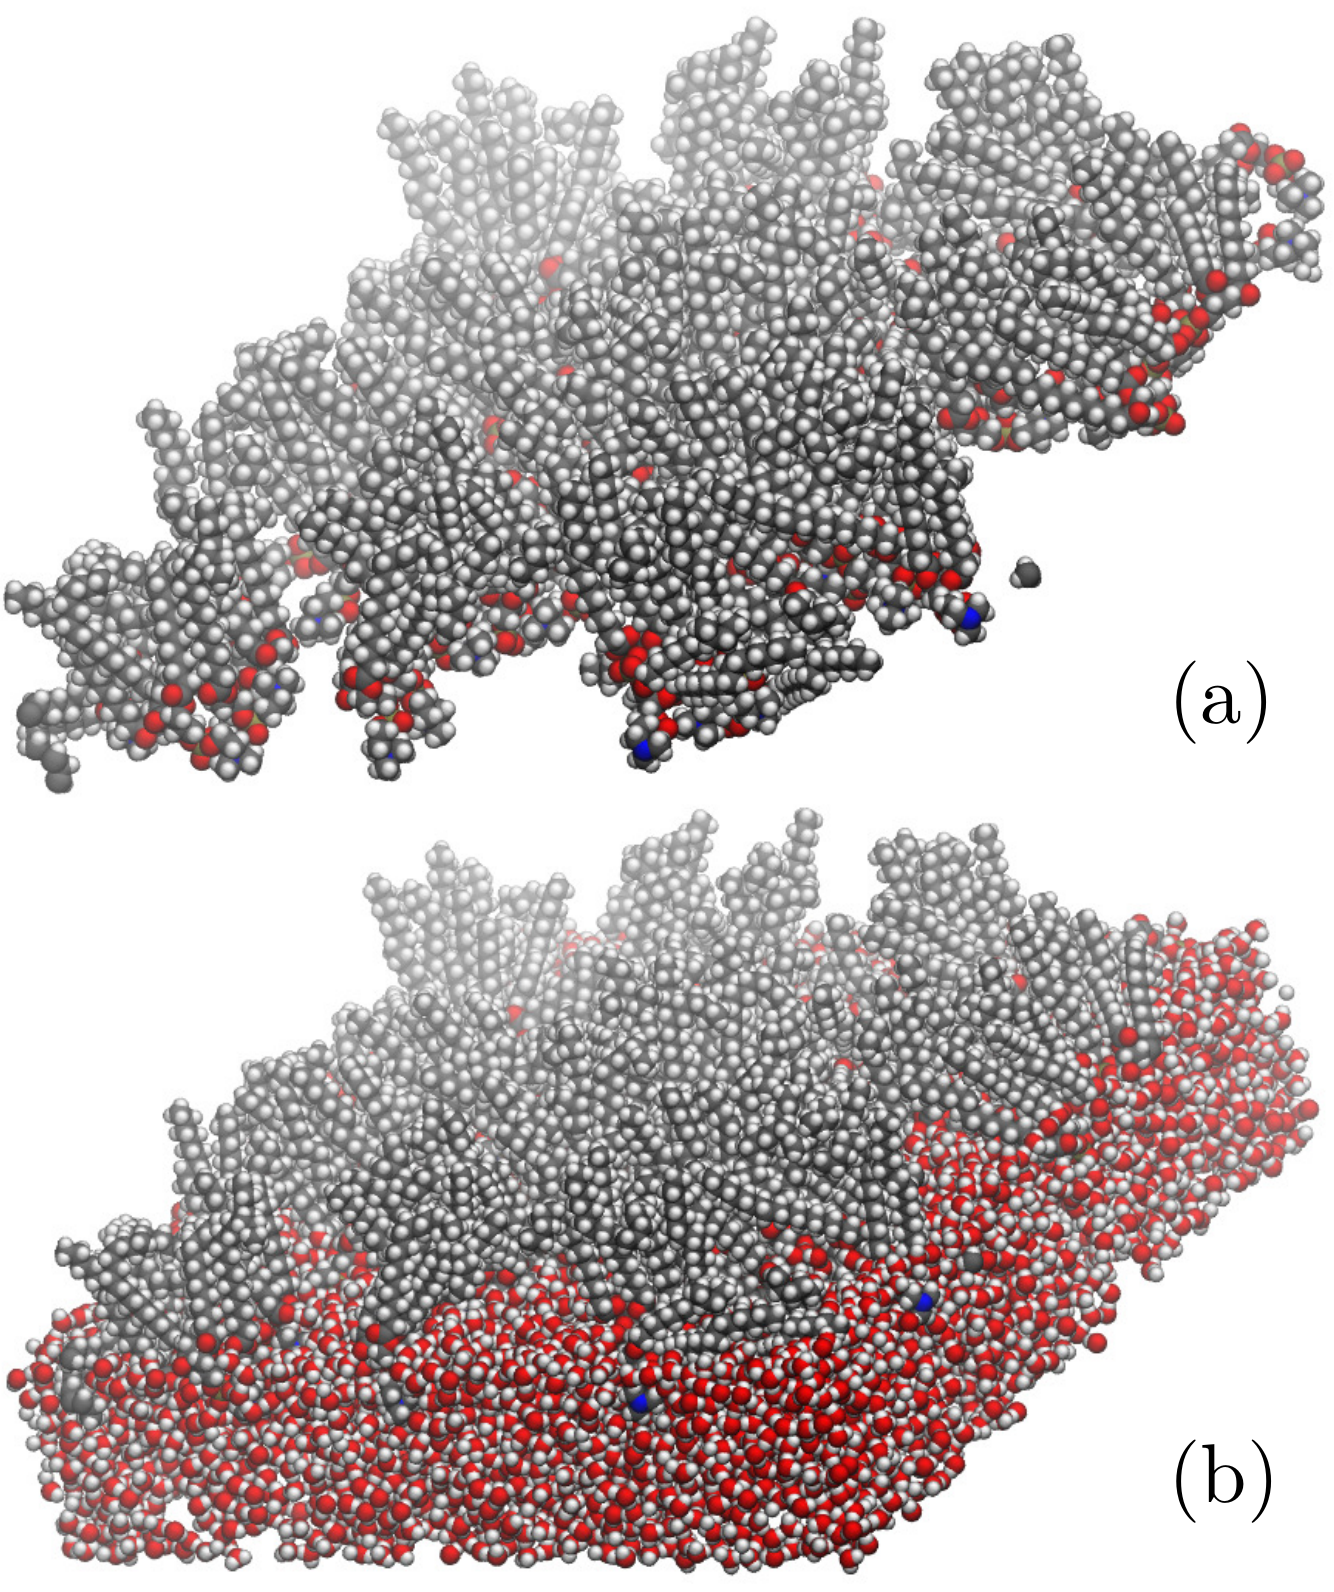
\includegraphics[width=0.4\textwidth]{dspcdrywet}
  \caption{The DSPC monolayer (a) without water layer and (b) with water layer, visuallised using VMD\cite{Humphrey1996}.}
  \label{fig:drywet}
\end{figure}
%
%
\begin{figure}[h]
\centering
  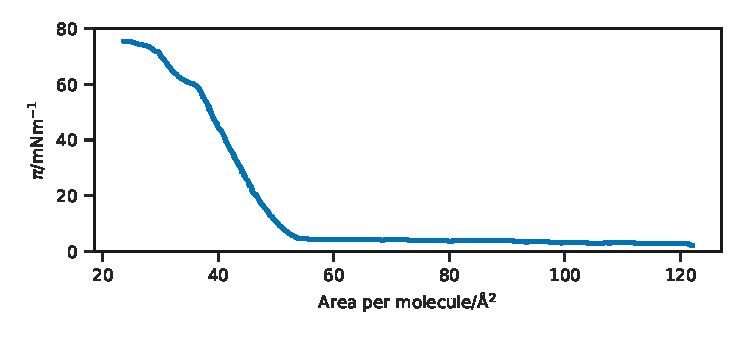
\includegraphics[width=0.48\textwidth]{apm}
  \caption{The experimental surface pressure isotherm for DSPC, taken from the work of Kubo \emph{et al.}\cite{Kubo2001}.}
  \label{fig:iso}
\end{figure}
%
%
\begin{table}[h]
\small
  \caption{\ The areas per molecule (APM) associated with particular surface pressures and the size of the \emph{x}- and \emph{y}-cell dimension for a simulation of 100 lipid molecules.}
  \label{tbl:apm}
  \begin{tabular*}{0.48\textwidth}{@{\extracolsep{\fill}}lll}
    \hline
    $\pi$/\si{\milli\newton\per\meter} & APM/\si{\angstrom\squared} & \emph{xy}-cell length/\si{\angstrom} \\
    \hline
    20 & 47.9 & 69.1 \\
    30 & 46.4 & 68.1 \\
    40 & 45.0 & 67.1 \\
    50 & 44.6 & 66.0 \\
    \hline
  \end{tabular*}
\end{table}
%

\subsection{Abel\`{e}s matrix formalism}
To compare against the simulation-derived reflectometry profiles, the chemically-consistent surfactant monolayer model was used \cite{McCluskey2018,McCluskey2018a}.
This model is implemented as a class that is compatible with the Python package refnx \cite{Nelson2018,refnx}.
The model is made up of two layers; the head-layer at the interface with the solvent and the tail-layer at the interface with the air.
The head components have a calculated scattering length, $b_h$, (found as a summation of the neutron scattering lengths of the individual atoms, see Table S1) and a component volume, $V_h$.
These make up a head-layer with a given thickness, $d_h$, and interfacial roughness, $\sigma_h$, and within this layer some volume fraction of solvent may intercalate, $\phi_h$.
The tail components also have a similarly calculated scattering length, $b_t$, and component volume, $V_t$.
This tail-layer also has a given thickness, $d_t$, and interfacial roughness, $\sigma_t$.
A maximum value for the thickness of the tail-layer was imposed, this value was taken from the Tanford Equation \cite{Tanford1980},
%
\begin{equation}
  t_t = 1.54 + 1.265n,
\end{equation}
%
where $n$ is the number of carbon atoms in the chain, and so for DSPC $t_t = \SI{24.3}{\angstrom}$.
The SLD of the tail and head layers used in the Abel\`{e}s matrix formalism can therefore be found as,
%
\begin{equation}
  \text{SLD}_i = \frac{b_i}{V_i}(1 - \phi_i) + \text{SLD}_s(\phi_i),
\end{equation}
%
where, $\text{SLD}_s$ is the scattering length density of the subphase (water), and $i$ indicates either the tail- or head-layer; it is assumed that the tail layer contains no solvent or air, e.g. $\phi_t = 0$ in agreement with the work of Campbell \emph{et al.} \cite{Campbell2018}.
To ensure that the number density of the head components and pairs of tail components is the same, the following constraint was included in the model \cite{Braun2017},
%
\begin{equation}
  \phi_h = 1 - \bigg(\frac{d_tV_h}{V_td_h}\bigg).
\end{equation}
%
A single value for the interfacial roughness was fit for all interfaces, as there is only a single lipid type in each monolayer \cite{Campbell2018}.
Therefore, any conformal roughness at the air-water interface is carried equally through all the layers.
The only modification made to this monolayer model used previously was that the tail component volume was also constrained, based on the APM (taken from the surface pressure isotherm),
%
\begin{equation}
  V_t = d_t \text{APM}.
\end{equation}
%
The result of this is that both the monolayer model and the simulation-derived models were constrained equally by this calculated surface coverage.

In this work, the experimental data from all seven contrasts were co-refined to a single monolayer model, where the head thickness, tail thickness, head component volume, and interfacial roughness were allowed to vary.
The values of the head and tail scattering lengths, along with the super and subphase SLDs are given in Table S1.
For each co-refinement of seven neutron reflectometry measurements, there were in total five degrees of freedom in the fitting process.
The Abel\`{e}s matrix formalism was used to calculate the reflectometry profiles as described in the ESI.

\subsection{Simulation-derived analysis}
Version 1.0.1 of refnx \cite{Nelson2018,refnx} includes the ability to obtain simulation-derived reflectometry profiles, using a similar method to that employed in previous work, such as Dabkowska \emph{et al.} \cite{Dabkowska2014}.
The Abel\`{e}s matrix formalism is applied to layers (see ESI), the SLD of which is drawn directly from the simulation, and the thickness of which is defined.
The layer thickness used was \SI{1}{\angstrom} for the Slipid and Berger potential model simulations, with an interfacial roughness between these layers is defined as \SI{0}{\angstrom}.
For the MARTINI potential model, a layer thickness of \SI{4}{\angstrom} was used, with an interfacial roughness of \SI{0.8}{\angstrom}, a detailed discussion for the rationale behind this is available in the ESI.
Each of the \SI{50}{\nano\second} production simulations were analysed with a frequency of every \SI{0.1}{\nano\second}, and the SLD profiles were determined by summing the scattering lengths, $b_j$, for each of the atoms in a given layer.
%
\begin{equation}
  \text{SLD}_n = \frac{\sum_j{b_j}}{V_n},
\end{equation}
%
where, $V_n$ is the volume of the layer $n$, obtained from the simulation cell parameters in the plane of the interface and the defined layer thickness.
A uniform background and scale factor were then determined using refnx to offer the best agreement between the calculated reflectometry profile and that measured experimentally.

\subsection{Comparison between monolayer model and simulation-derived analysis}
\label{sec:para}
In order to assess the agreement between the models from each method, the following goodness-of-fit metric was used, following the transformation of the data into $Rq^4$ space,
%
\begin{equation}
  \chi^2 = \sum_{i=1}^{N_{\text{data}}} \frac{[R_{\text{exp}}(q_i) - R_{\text{sim}}(q_i)]^2}{[\delta R_{\text{exp}}(q_i)]^2},
\end{equation}
%
where $q_i$ is a given $q$-vector, which depends on the neutron wavelength and reflected angle, $R_{\text{exp}}(q_i)$ is the experimental reflected intensity, $R_{\text{sim}}(q_i)$ is the simulation-derived reflected intensity, and $\delta R_{\text{exp}}(q_i)$ is the resolution function of the data.

Parameteric outcomes from the different analysis methods were also compared, such as the number of water molecules per head group, wph.
This was obtained from the monolayer model by considering the solvent fraction in the head-layer, $\phi_h$, the volume of the head group, $V_h$, and taking the volume of a single water molecule to be \SI{29.9}{\cubic\angstrom} (from the density of water as \SI{997}{\kilo\gram\per\cubic\meter}),
%
\begin{equation}
  \text{wph} = \frac{\phi_hV_h}{29.9 - 29.9\phi_h}.
  \label{equ:wph}
\end{equation}
%
From the molecular dynamics simulation, the number densities for each component of the system were determined.
The ratio of the integrals of the lipid heads and the water then gave the wph.
The range for this integral was taken as between the \SI{20}{\percent} and \SI{80}{\percent} quantiles of the lipid head-layers.

\section{Results \& Discussion}
%
\begin{figure*}
 \centering
 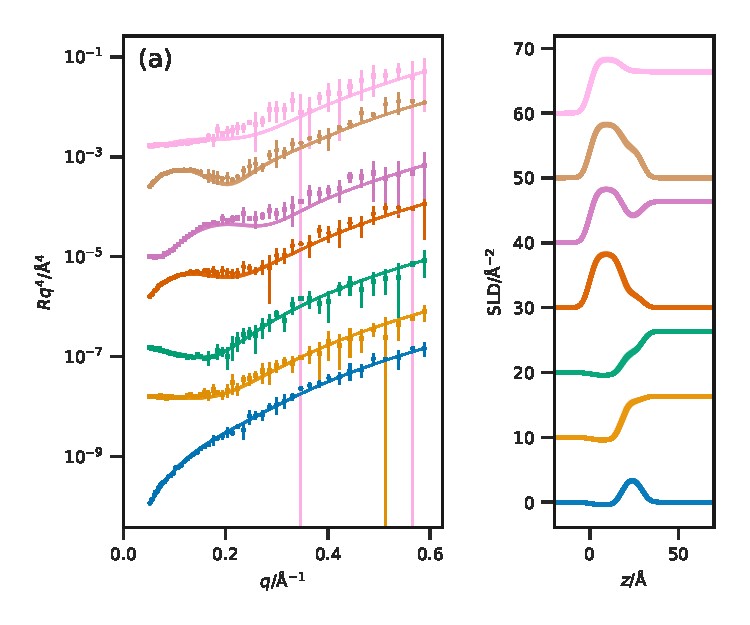
\includegraphics[width=0.49\textwidth]{trad_30}
 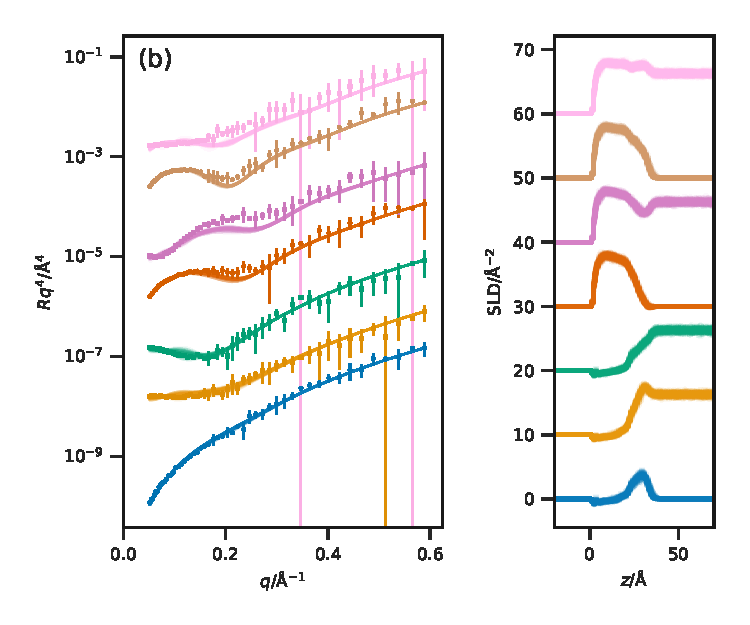
\includegraphics[width=0.49\textwidth]{sim_slipids_30} \\
 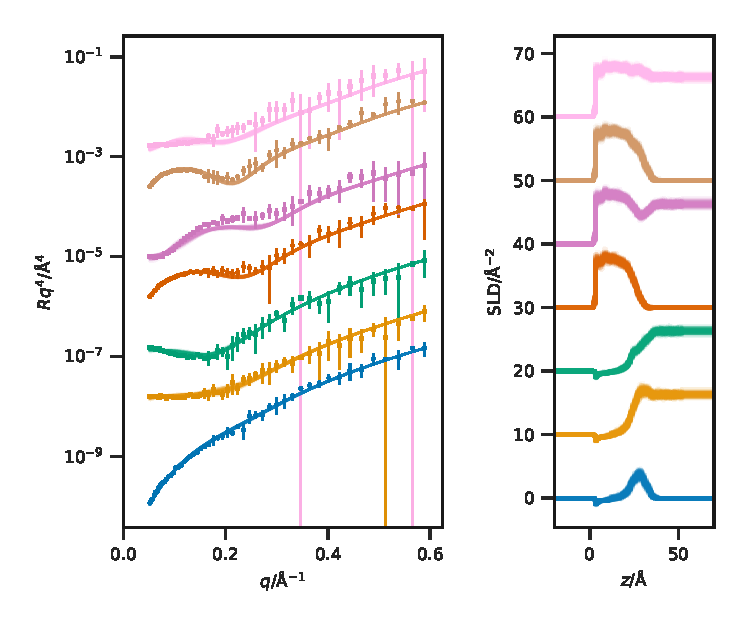
\includegraphics[width=0.49\textwidth]{sim_berger_30}
 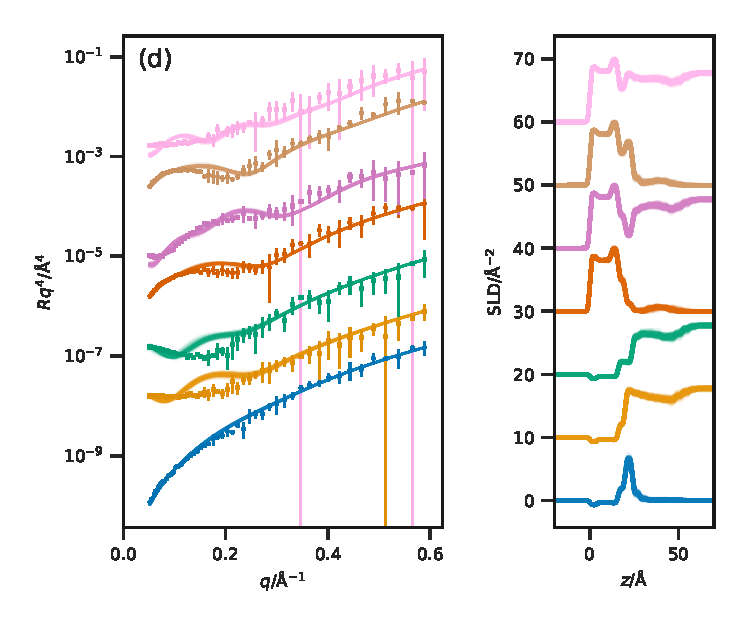
\includegraphics[width=0.49\textwidth]{sim_martini_30}
 \caption{A comparison of the reflectometry and SLD profiles obtained from (a) the monolayer model, (b) the Slipid simulation, (c) the Berger force-force simulation, and (d) the MARTINI potential model simulation at a surface pressure of \SI{30}{\milli\newton\per\meter}. From top-to-bottom the contrasts are as follows; \ce{d_{83}}-\ce{D2O}, \ce{d_{83}}-ACMW, \ce{d_{70}}-\ce{D2O}, \ce{d_{70}}-ACMW, h-\ce{D2O}, \ce{d_{13}}-\ce{D2O}, \ce{d_{13}}-ACMW. The different contrast reflectometry profiles have been offset in the \emph{y}-axis by an order of magnitude and the SLD profiles offset in the \emph{y}-axis by \SI{1e-6}{\per\square\angstrom}, for clarity.}
 \label{fig:ref}
\end{figure*}
%
Figure \ref{fig:ref} compares the reflectometry and SLD profiles from each of the different methods used at a surface pressure of \SI{30}{\milli\newton\per\meter}.
The data for the other surface pressures showed similar trends, and can be found in the ESI.
The $\chi^2$ goodness-of-fit metric between the calculated and experimental reflectometry is given in Table \ref{tbl:chi} for each contrast, in addition to the average $\chi^2$ and a standard deviation.
%
\begin{table*}
\small
  \caption{\ The goodness-of-fit between the calculated and experimental reflectometry profile at a surface pressure of \SI{30}{\milli\newton\per\metre}.}
  \label{tbl:chi}
  \begin{tabular*}{\textwidth}{@{\extracolsep{\fill}}lllll}
    \hline
    Contrast & Monolayer model & Slipid & Berger & MARTINI \\
    \hline
    h-\ce{D2O} & \input{../output/traditional/hd2o_30_chisq.txt} & \input{../output/simulation/hd2o_slipids_30_chisq.txt} & \input{../output/simulation/hd2o_berger_30_chisq.txt} & \input{../output/simulation/hd2o_martini_30_chisq.txt} \\
    \ce{d_{13}}-ACMW & \input{../output/traditional/d13acmw_30_chisq.txt} & \input{../output/simulation/d13acmw_slipids_30_chisq.txt} & \input{../output/simulation/d13acmw_berger_30_chisq.txt} & \input{../output/simulation/d13acmw_martini_30_chisq.txt} \\
    \ce{d_{13}}-\ce{D2O} & \input{../output/traditional/d13d2o_30_chisq.txt} & \input{../output/simulation/d13d2o_slipids_30_chisq.txt} & \input{../output/simulation/d13d2o_berger_30_chisq.txt} & \input{../output/simulation/d13d2o_martini_30_chisq.txt} \\
    \ce{d_{70}}-ACMW & \input{../output/traditional/d70acmw_30_chisq.txt} & \input{../output/simulation/d70acmw_slipids_30_chisq.txt} & \input{../output/simulation/d70acmw_berger_30_chisq.txt} & \input{../output/simulation/d70acmw_martini_30_chisq.txt} \\
    \ce{d_{70}}-\ce{D2O} & \input{../output/traditional/d70d2o_30_chisq.txt} & \input{../output/simulation/d70d2o_slipids_30_chisq.txt} & \input{../output/simulation/d70d2o_berger_30_chisq.txt} & \input{../output/simulation/d70d2o_martini_30_chisq.txt} \\
    \ce{d_{83}}-ACMW & \input{../output/traditional/d83acmw_30_chisq.txt} & \input{../output/simulation/d83acmw_slipids_30_chisq.txt} & \input{../output/simulation/d83acmw_berger_30_chisq.txt} & \input{../output/simulation/d83acmw_martini_30_chisq.txt} \\
    \ce{d_{83}}-\ce{D2O} & \input{../output/traditional/d83d2o_30_chisq.txt} & \input{../output/simulation/d83d2o_slipids_30_chisq.txt} & \input{../output/simulation/d83d2o_berger_30_chisq.txt} & \input{../output/simulation/d83d2o_martini_30_chisq.txt} \\
    \hline
    Average$\pm$Uncertainty & \input{../output/traditional/ave_30_chisq.txt} & \input{../output/simulation/ave_slipids_30_chisq.txt} & \input{../output/simulation/ave_berger_30_chisq.txt} & \input{../output/simulation/ave_martini_30_chisq.txt} \\
    \hline
  \end{tabular*}
\end{table*}
%

\subsection{Comparison of MARTINI}
It is clear from Figure \ref{fig:ref} and Table \ref{tbl:chi}, that the MARTINI potential model simulations very poorly reproduce the reflectometry profile.
Furthermore, it is noted that the agreement with the contrasts containing \ce{D2O} are particularly poor.
This is most likely an artefact of the structuring effect from the wall at the bottom of the simulation cell on the polarisable MARTINI water.
It is noted that this may be reduced through the use of a less-ordered wall structure \cite{Koutsioubas2016}.
Another outstanding artefact present in the MARTINI potential model simulations is that the calculated length of the hydrocarbon tail from the simulation was found to be \input{../output/simulation/martini_30_tt.txt}\si{\angstrom}, which is significantly less than the \SI{24.3}{\angstrom} estimated by the Tanford equation.
This is due to the nature of the MARTINI's 4-to-1 beading process, as DSPC has a hydrocarbon tail consisting of 18 carbon atoms, not possible to bead such a chain accurately with the MARTINI potential model..
In this work, a MARTINI lipid molecule was used with 4 MARTINI beads making up the chain; corresponding to an all-atom hydrocarbon chain of 16 atoms.
Applying the Tanford equation to a hydrocarbon chain of such a length results in an anticipated length of \SI{18.7}{\angstrom}, which agrees better with that found from simulation.

The requirement for a 4-to-1 beading structre of the MARTINI potential model is a significant weakness in this work.
A better method may involve the use of a 2-to-1 beading model.
However, we are not aware of an off-the-shelf 2-to-1 coarse-grained potential model that is commonly applied to lipid molecules.

\subsection{Comparison of other simulations}
Table \ref{tbl:chi} shows that both the Slipid and Berger potential models agree well with the experimental data, with the Slipid potential model offering a slight improvement over the Berger.
The quality of agreement between these higher-resolution potential models and the monolayer model is relatively similar.
However, the monolayer model is still better than those determined from MD simulation.
This is to be expected though, simply by considering the level of constraint present implicitly when determining the reflecometry profile directly from simulation.
While the monolayer model constrains the layer model to be chemically-consistent, those from MD simulation have real chemical constraints present in the simulation; e.g. the bonding of atoms, and the non-bonded potentials.
The quality of the agreement from this multi-modal analysis technique it sufficient for such a method to be applied regularly in the analysis of neutron reflectometry.

Both the Slipid and Berger simulations produced values for the tail length that were in better agreement with the Tanford equation than the MARTINI simulation.
For the Slipid simulation the tail length was found to be \input{../output/simulation/slipids_30_tt.txt}\si{\angstrom}, while for the Berger simulations a value of \input{../output/simulation/berger_30_tt.txt}\si{\angstrom} was obtained.
Neither is quite as large as the \SI{24.3}{\angstrom} from the Tanford equation, however it should be noted that this value is considered a maximum for the \emph{fully extended} carbon tail.

Using the molecular dynamics simulations, and the monolayer model it is possible to compare the number of water molecules per head group.
From the Slipids and Berger simulations, the number of water molecules per head group was found to be \input{../output/simulation/slipids_30_wph.txt} and \input{../output/simulation/berger_30_wph.txt} respectively.
These are in good agreement with the \input{../output/traditional/wph_30.txt} found from the monolayer model method in conjungtion with Equation \ref{equ:wph}.

It should be noted that to obtain the \SI{50}{\nano\second} production run for the Slipids potential model simulation required over 13 days of using 32 cores of the SCARF computing resource.
This is non-trivial and therefore not necessarily applicable to all neutron reflectometry measurements.
However, for the nearly as accurate Berger potential model simulations (which are only marginally less accurate), only approximately 2 days, of the same compute resource, were required.
This suggests that given the quality of agreement with the experimental data achieved from the Berger potential model simulations it may be feasible to suggest simulations of such resolution may be run alongside experimental measurements at large facilities such as ISIS Neutron and Muon Source.

\subsection{Using the Slipid simulations to improve the monolayer model}
Despite the monolayer model offering a small improvement in agreement over the Slipid potential model simulation, we believe that it is possible to use these MD simulations to improve the existing monolayer model.
An example of this has already been mentioned in terms of not applying the assumption that the carbon tail is fully extended.
Another possible improvement can be found by considering Figure \ref{fig:nb}, which shows the water molecules per head group as a function of depth; it is clear that solvent penetration into the lipid head group area is not uniform.
In particular, there is a clear pocket of water formed around the ester group of the lipid.
This suggests that perhaps a different model for solvent penetration could be applied to the head layer to better describe the realistic solvent penetration.
%
\begin{figure}
\centering
  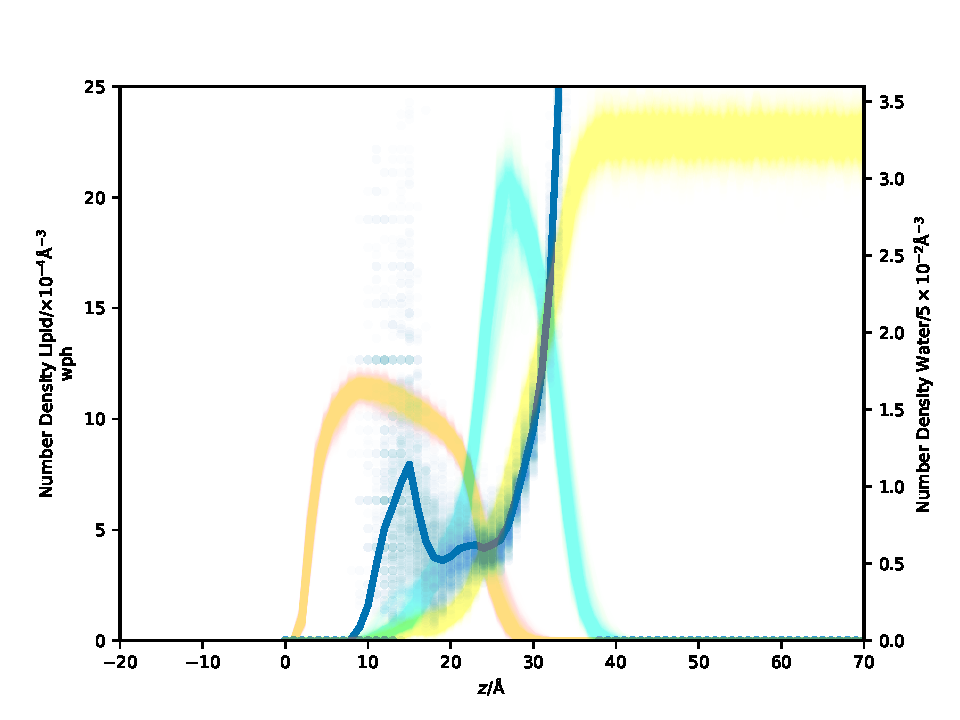
\includegraphics[width=0.48\textwidth]{number_density}
  \caption{The number density of each component; tails (orange), heads (green), water (yellow), and the number of water molecules per head group (blue dots, with the time-average shown as a solid blue line).}
  \label{fig:nb}
\end{figure}
%

It is generally suggested that the conformal roughness between layers should be carried evenly through the monolayer when there is only a single lipid type \cite{Campbell2018}.
However, from Figure \ref{fig:nb} it is clear that the overlap between the head-layer and water is much larger than that between the tail and head.
Furthermore, there is additionally some solvent present deep within the tail layer, due to the presence of head-group character in that region.
While the interfacial roughness can be considered as describing the capillary wave form of the water surface, it is also frequently applied to account for the intrinsic/structural roughness in the monolayer that exists because of the fact that the lipid ensemble comprises molecules with different conformations and thus different chain lengths.
This suggests that perhaps the constraint that the interfacial roughnesses should be constant through the monolayer might be relaxed.


\section{Conclusions}
This work presented, for the first time, direct comparison between a traditional method for analysis of neutron reflectometry measurement with analysis derived from a range of all-atom and coarse-grained molecular dynamics simulations; using the all-atom Slipid, the united-atom Berger, and the coarse-grained MARTINI potential models.
It was found that the MARTINI potential model is not capable of accurately modelling the lipid monolayer system due to the limitations of the 4-to-1 beading system when applied to a carbon tail containing 18 atoms.
The Berger and Slipid potential models both showed good agreement with the experimental data, however the best agreement was obtained by the traditional monolayer model.
This would be expected given that the monolayer model contains many more degrees of freedom than the simulations which are severely chemically constrained by the potential model.
Finally, some points from the highest resolution, Slipid, simulations were noted that may be used to improve the traditional monolayer model.
These include the fact that the carbon tails were not always fully extended, and the possible desire for a non-uniform solvation of the head group region.

\section{Author Contributions}
The initial experiments were conducted by D.J.B. and M.J.L..
The analysis methodology was developed by A.R.M. with input from J.G., A.J.S., J.L.R., S.C.P. and K.J.E..
A.R.M. wrote the manuscript, with input from all authors.

\acknowledgements{
ARM is grateful to the University of Bath and Diamond Light Source for co-funding a studentship (Studentship Number STU0149). This work benefited from the computing resources provided by STFC Scientific Computing Department's SCARF cluster.
We thank Robert D. Barker for insightful discussion.}

\bibliography{paper.bib}


\end{document}                    % DO NOT DELETE THIS LINE
